\section*{Question}

A random point $(X,Y)$ is chosen in the following square:
\begin{align*}
    \{(x, y) : x^2 < e,  y^2 < e \}
\end{align*}
All points are equally likely to be chosen. Let $S$ be the Euclidean norm of $(X,Y)$.
\begin{exercise}[1]
Find the joint PDF $f(x,y)$ of $X$ and $Y$.
\begin{solution}
Since $(X,Y)$ is uniformly distributed on $(-\sqrt{e}, \sqrt{e})^2$, their joint PDF is simply:
\begin{align*}
    f(x,y) =& \Big(\frac{1}{\sqrt{e} - (-\sqrt{e}))} \Big) \Big(\frac{1}{(\sqrt{e} - (-\sqrt{e}))} \Big) \\
    =& \frac{1}{4e},
\end{align*}\\
for $x\in (-\sqrt{e}, \sqrt{e})$ and $y\in (-\sqrt{e}, \sqrt{e})$.
\textit{0.5 points for the solution, 0.5 points for the correct bounds.}
\end{solution}
\end{exercise}


\begin{exercise}[3]
Find the expectation of $S^2$, i.e., the squared norm of $(X,Y)$.
\begin{solution}
Note that $S = X^2 + Y^2$. Using LOTUS and symmetry in $x$ and $y$:
\begin{align*}
      \int_{-\infty}^\infty \int_{-\infty}^\infty \Big(x^2 + y^2 \Big) f(x,y) \; dx \; dy =& \int_{-\sqrt{e}}^{\sqrt{e}} \int_{-\sqrt{e}}^{\sqrt{e}}  \Big(x^2 + y^2 \Big) \Big(\frac{1}{4e} \Big) \; dx \; dy \\
      =& \frac{1}{4e} \int_{-\sqrt{e}}^{\sqrt{e}} \int_{-\sqrt{e}}^{\sqrt{e}} (x^2 + y^2) \; dx \; dy \\
      =& \frac{1}{4e} \int_{-\sqrt{e}}^{\sqrt{e}} \int_{-\sqrt{e}}^{\sqrt{e}} x^2 \; dx \; dy + \frac{1}{4e} \int_{-\sqrt{e}}^{\sqrt{e}} \int_{-\sqrt{e}}^{\sqrt{e}} y^2 \; dx \; dy + \\
      =& \frac{2}{4e} \int_{-\sqrt{e}}^{\sqrt{e}} \int_{-\sqrt{e}}^{\sqrt{e}} x^2 \; dx \; dy \\
      =& \frac{1}{2e} \int_{-\sqrt{e}}^{\sqrt{e}}  [\frac{1}{3} x^3]_{\sqrt{e}}^{\sqrt{e}} \; dy \\
      =& \frac{1}{6e} \int_{-\sqrt{e}}^{\sqrt{e}} (e^{3/2} + e^{3/2} ) \; dy \\
      =& \frac{2}{6e} 2\sqrt{e} e^{3/2}  \\
      =& \frac{4e^2}{6e} = \frac{2}{3}e.
\end{align*} \\
\textit{One point for finding $S^2 = X^2 + Y^2$ and writing down the integral correctly using LOTUS. Two points for the remaining calculations.}
\end{solution}
\end{exercise}
\noindent
Consider the following code:
\begin{minted}{python}
import numpy as np
import matplotlib.pyplot as plt
np.random.seed(3)

num = 10000

x = np.random.normal(loc = 1, scale = np.sqrt(2), size = num)
y = 10 - x

print(np.corrcoef(x,y))

plt.scatter(x,y)
\end{minted}

\begin{minted}{R}
set.seed(3)

num = 10000

x = rnorm(num, mean = 1, sd = sqrt(2))
y = 10 - x

print(cor(x,y))

plot(x,y)
\end{minted}

\begin{exercise}[1]
This code gives the value -1 and the following graph.
\begin{figure}[H]
    \centering
    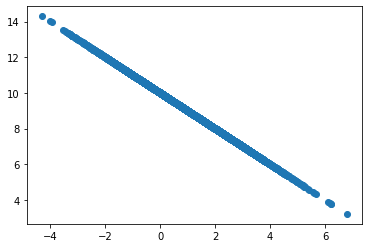
\includegraphics[width = 0.5 \textwidth]{plotexam.png}
\end{figure}
\noindent
Explain, what the relationship is between the numerical and graphical output and why the output is -1.
\begin{solution}
The output of -1 means that the correlation between $X$ and $Y$, is -1. This makes sense since $Y = 10 - X$, so obviously the correlation is -1 as $Y$ completely determines the value of $X$. If $Y$ goes up by 1, $X$ always goes down by exactly 1. This can also be seen in the graph where $X$ and $Y$ always sum op to 10 and there is are linear negative relationship between them. No points are deviated from the line, $X$ and $Y$ will always move together.
\end{solution}
\end{exercise}
